\chapter{Analyse de l'éxistant}
Use the ``quote'' and ``quotation'' environments for typesetting quoted
material or any other text that should be slightly indented and set off
from the normal text.
\begin{quotation}
The quote and quotation environments are similar, but use different
settings for paragraph indentation and spacing.

\em When in doubt, consult the manual.
\end{quotation}

So far, I have demonstrated titles, paragraphs, font changes, and
section headings.
%\includegraphics[width=\textwidth]{./pictures/general_view.png}

\begin{figure}[h!tb]
    \centering
    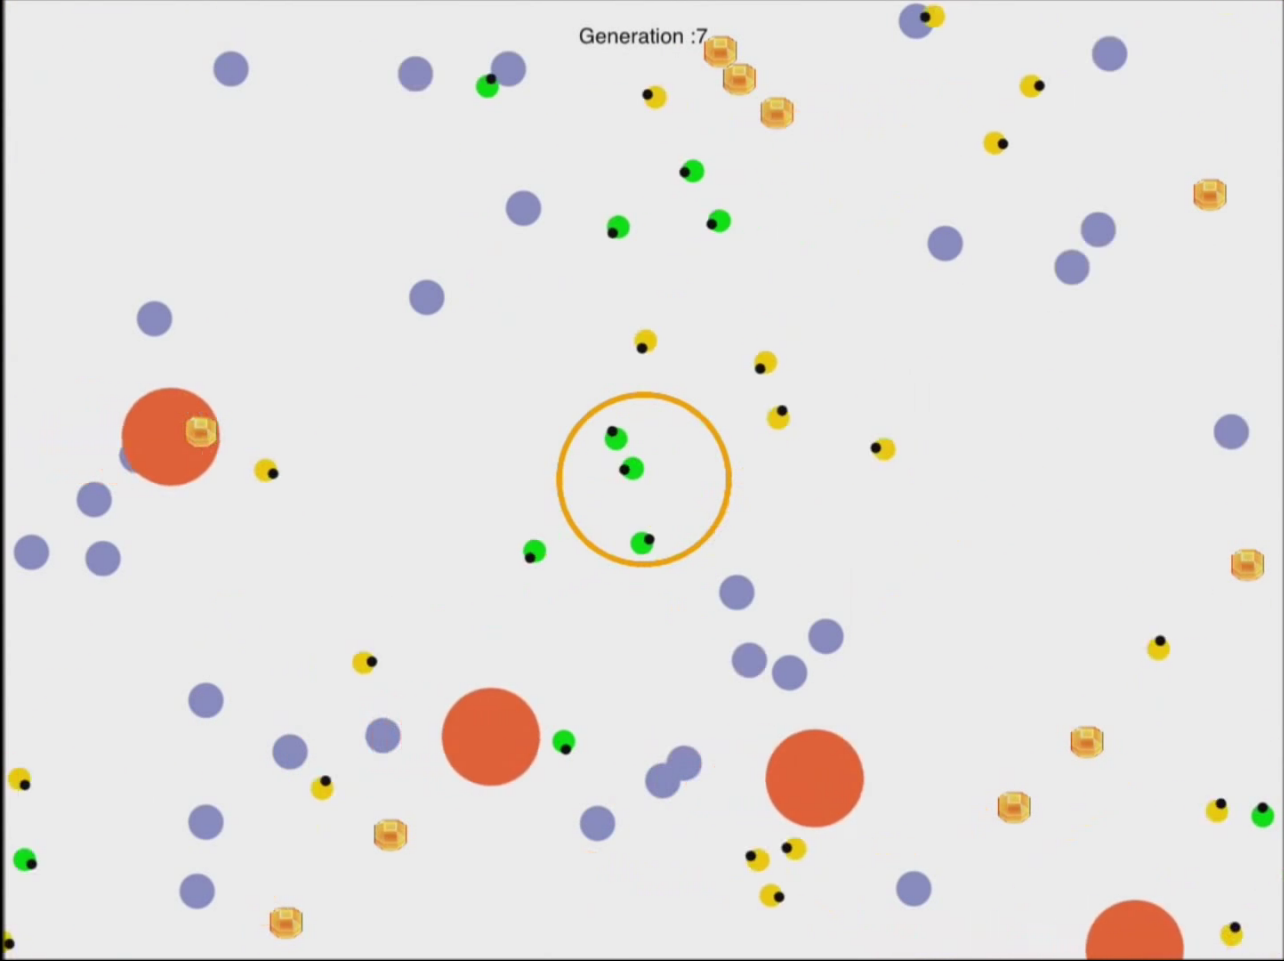
\includegraphics[width=0.8\textwidth]{./pictures/prototype.png}
    \caption{General view}
    \label{fig:awesome_image}
\end{figure}

Now, I am going to show lists and tables. 

\pagebreak
